% Template:     Informe LaTeX
% Documento:    Archivo de ejemplo
% Versión:      8.1.7 (24/07/2022)
% Codificación: UTF-8
%
% Autor: Pablo Pizarro R.
%        pablo@ppizarror.com
%
% Manual template: [https://latex.ppizarror.com/informe]
% Licencia MIT:    [https://opensource.org/licenses/MIT]

\section{Introducción}

\lipsum[2-4]

\section{Configuración de una instancia EC2}
\subsection{Inicio de sesión en AWS}

Se inicia sesión en AWS con la cuenta awsacademy en el siguiente url: \href{https://awsacademy.instructure.com/}{https://awsacademy.instructure.com/}

\begin{figure}[h]
	\centering
	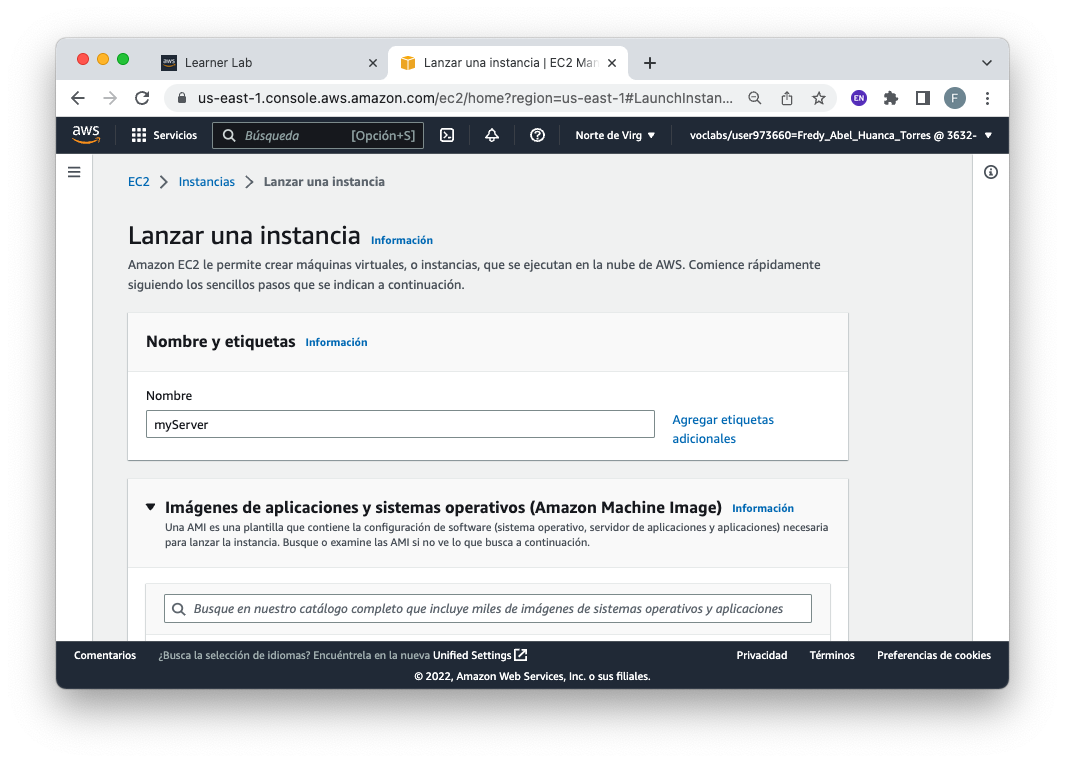
\includegraphics[scale=.3] {img/01}
	\caption{Inicio de sesión}
	\label{fig:0}	
\end{figure} 

\clearpage

\begin{figure}[h]
	\centering
	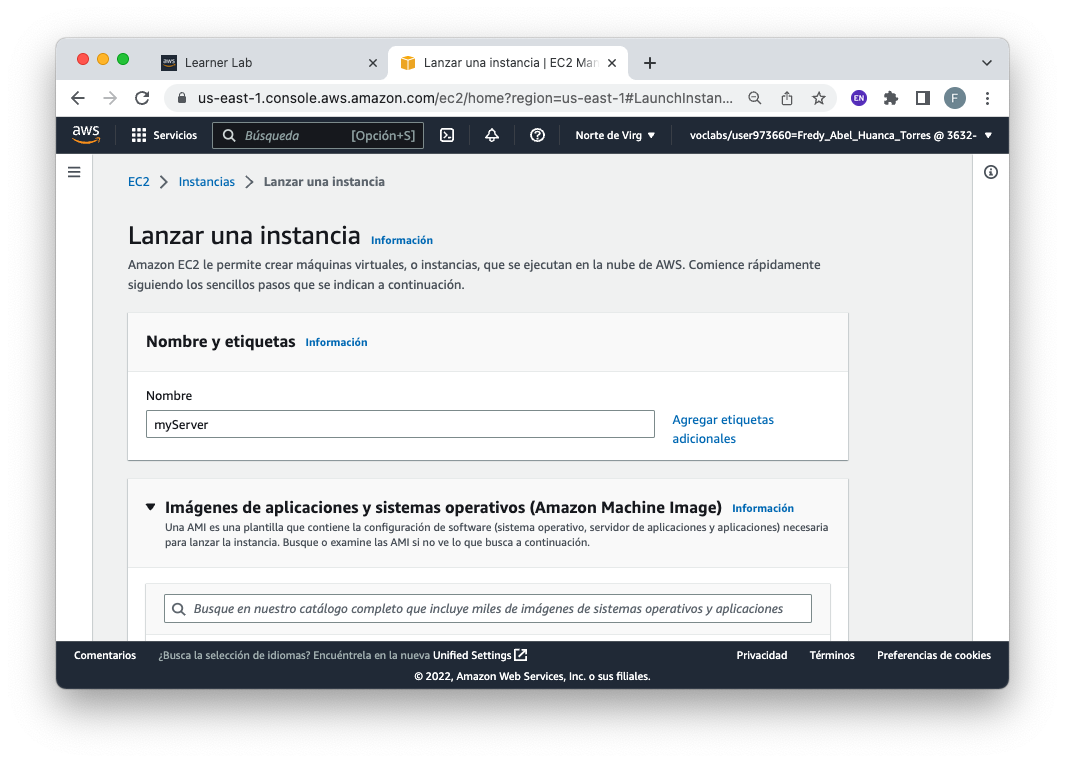
\includegraphics[scale=.3] {img/01}
	\caption{Creación de instancia ec2}
	\label{fig:1}	
\end{figure} 

Amazon EC2 le permite crear máquinas virtuales, o instancias, que se ejecutan en la nube de AWS. Comience rápidamente siguiendo los sencillos pasos que se indican a continuación.

\begin{figure}[h]
	\centering
	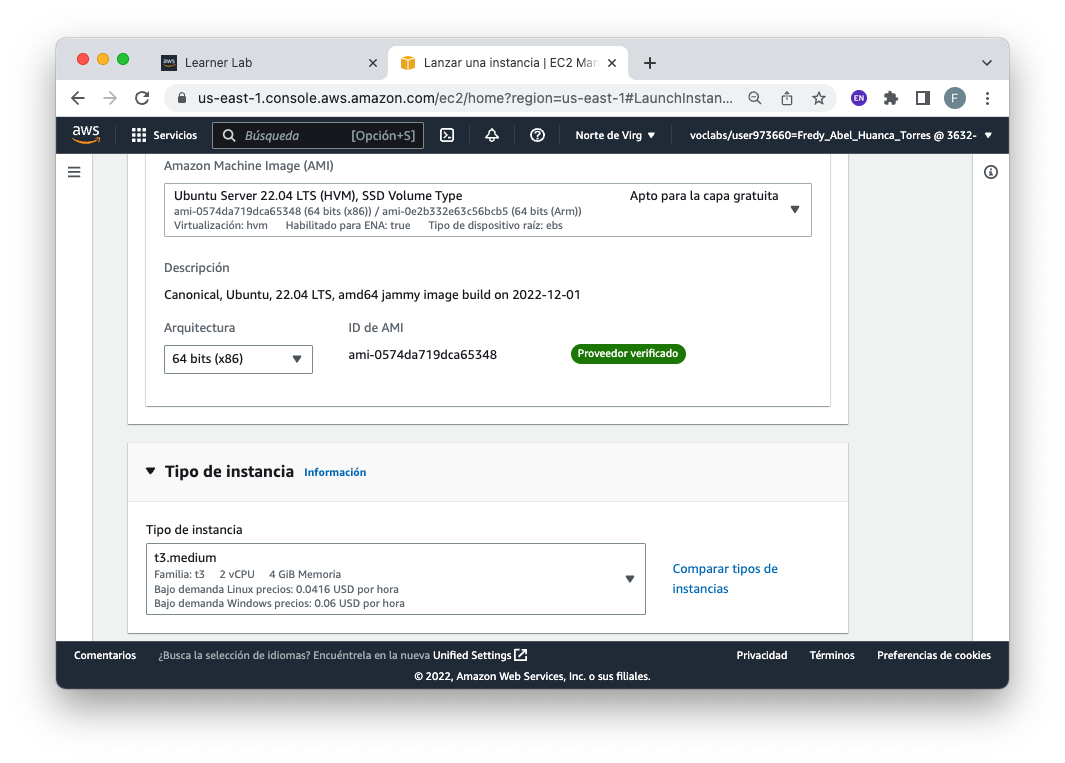
\includegraphics[scale=.3] {img/02}
	\caption{Par de claves: myKey.pem}
	\label{fig:2}	
\end{figure} 


\clearpage

\subsection{Selección de imagen AMI y tipo de instancia}

Amazon Machine Image (AMI) son imágenes que proporciona aws, y se seleccionó: Ubuntu Server 22.04 LTS (HVM).

\begin{figure}[h]
	\centering
	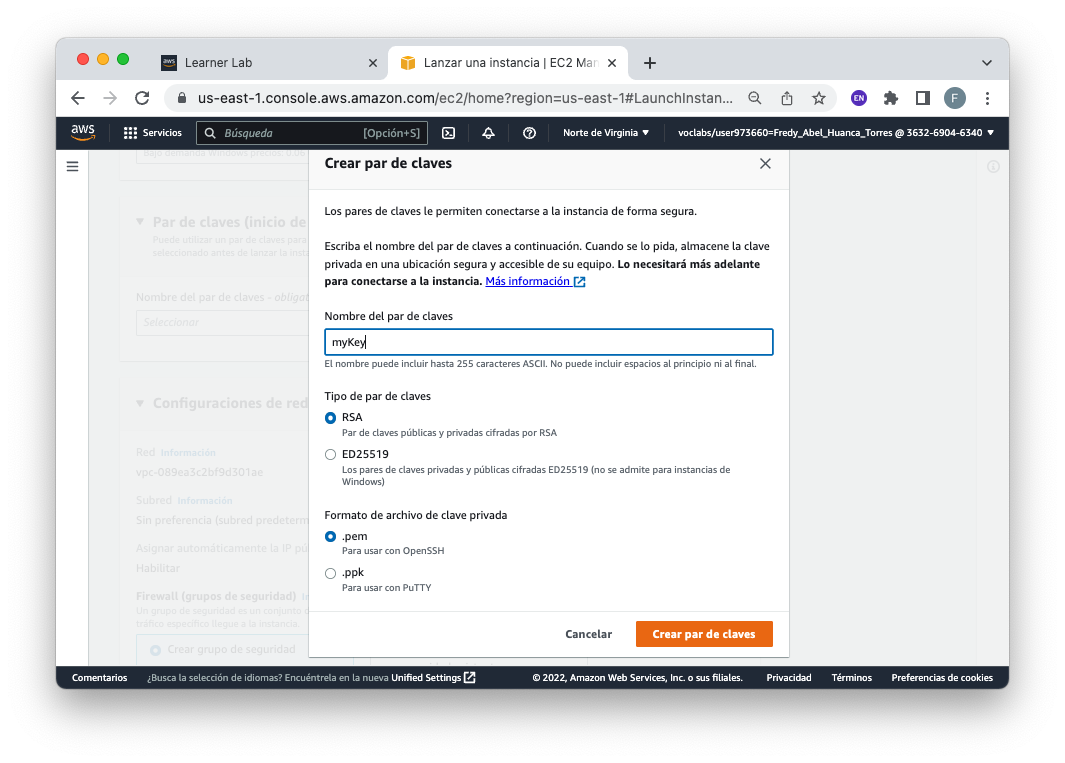
\includegraphics[scale=.3] {img/03}
	\caption{Imagen AMI Ubuntu 20.04, tipo: t3.medium}
	\label{fig:3}	
\end{figure}

\subsection{Configuración del Grupo de Seguridad}
Un grupo de seguridad es un conjunto de reglas de firewall  que controlan el trático de la instancia.
\begin{figure}[h]
	\centering
	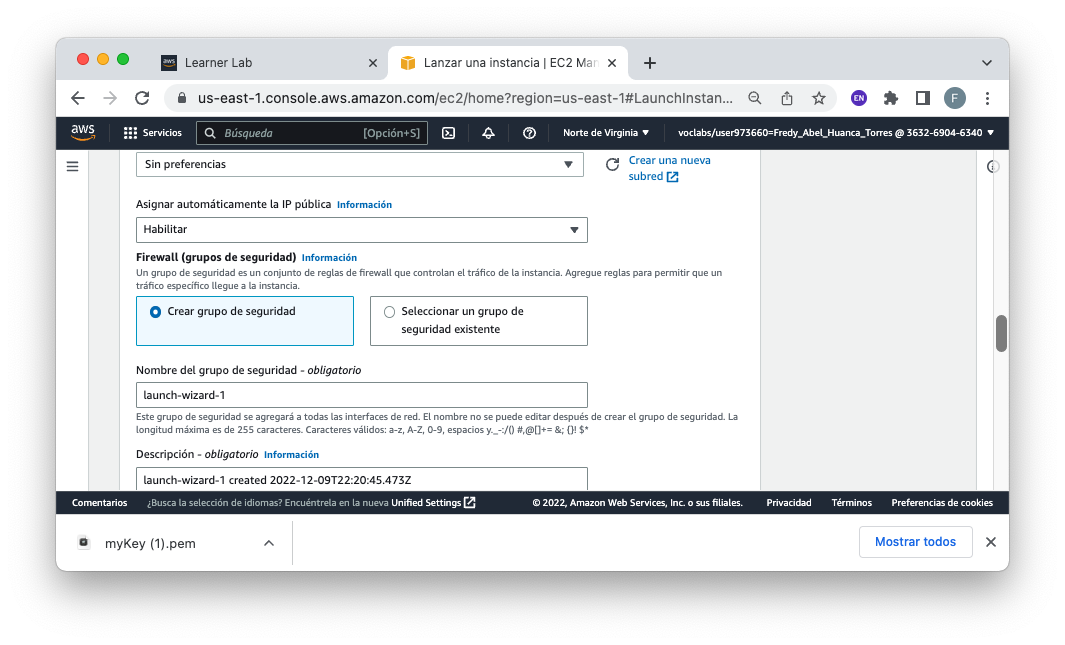
\includegraphics[scale=.35] {img/04}
	\caption{grupo de seguridad: habilitación de conexión ssh}
	\label{fig:4}	
\end{figure} 

\clearpage

\subsection{Iniciar instancia}
En esta sección se presenta el resumen de la instancia ec2 configurada. 
\begin{figure}[h]
	\centering
	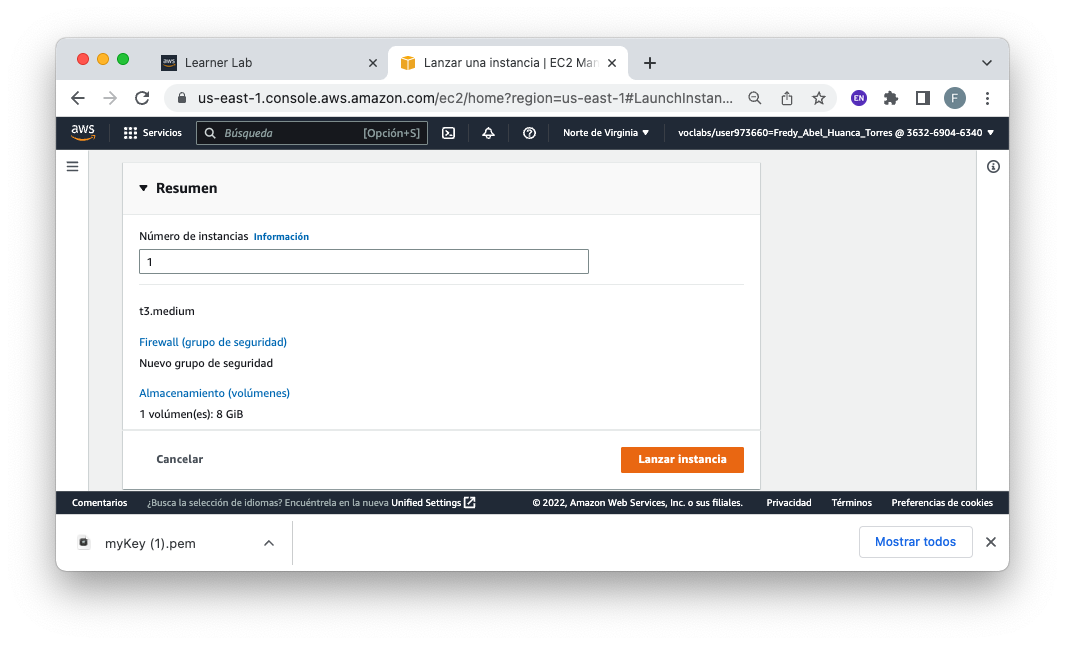
\includegraphics[scale=.35] {img/06}
	\caption{Resumen de instancia}
	\label{fig:6}	
\end{figure} 

La siguiente figura muestra la confirmación del lanzamiento de la instancia, indicando que se realizo de forma satisfactoria 
\begin{figure}[h]
	\centering
	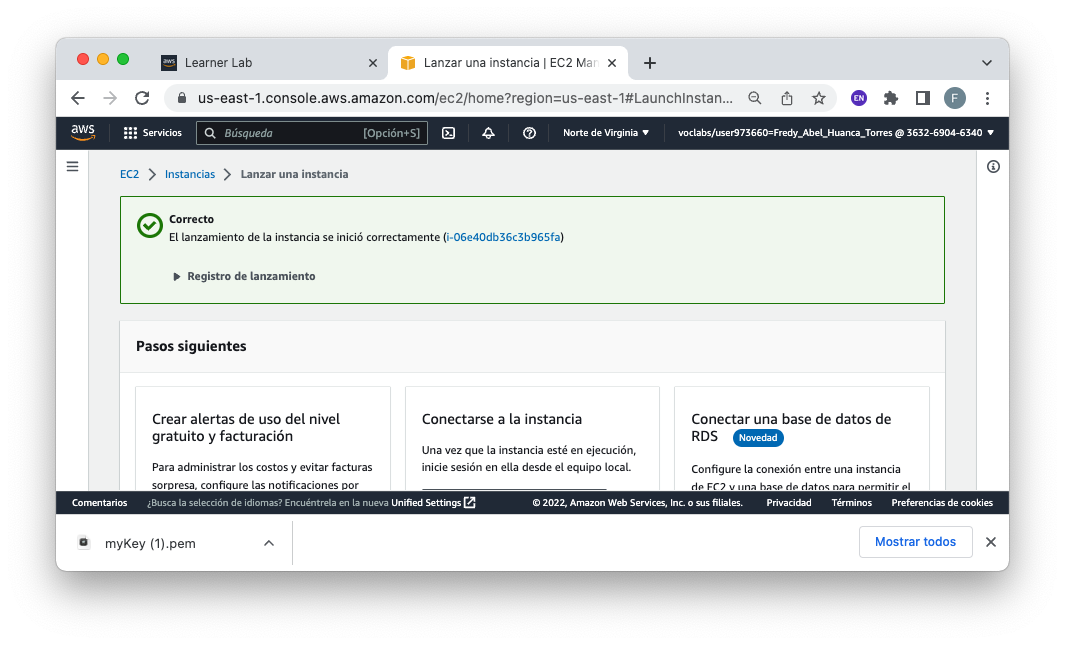
\includegraphics[scale=.35] {img/07}
	\caption{Instancia ejecutándose de manera satisfactoria}
	\label{fig:7}	
\end{figure} 

\clearpage

Consola de aws donde se muestra la lista de instancias creadas y demás metadatos asociados a los mismo. 
\begin{figure}[h]
	\centering
	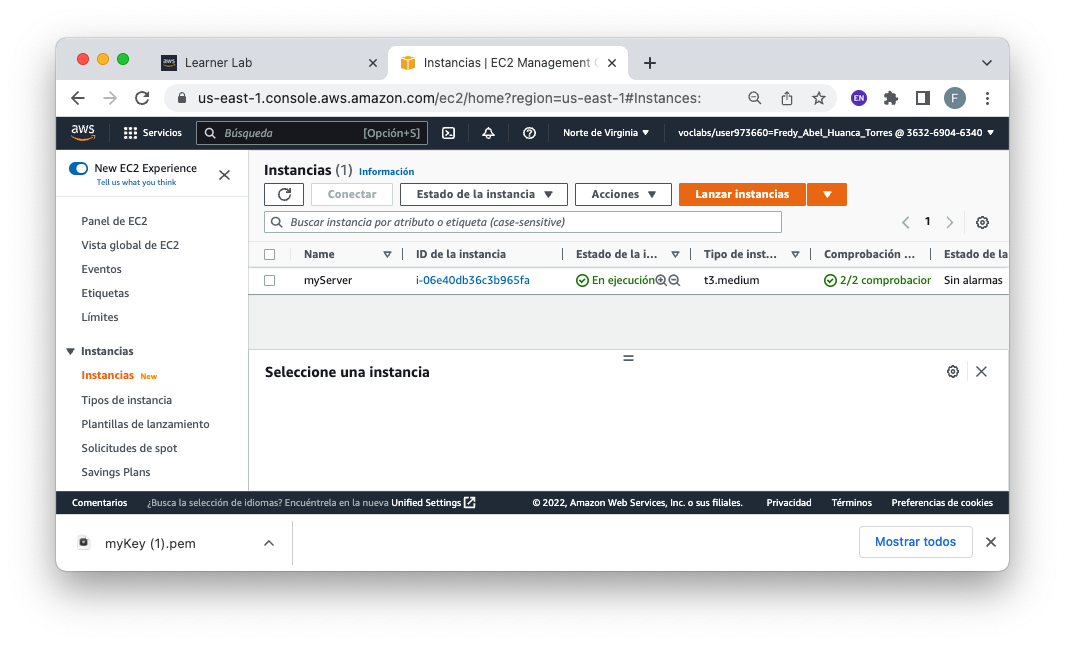
\includegraphics[scale=.35] {img/08}
	\caption{Lista de instancias en ejecución}
	\label{fig:8}	
\end{figure} 

\begin{figure}[h]
	\centering
	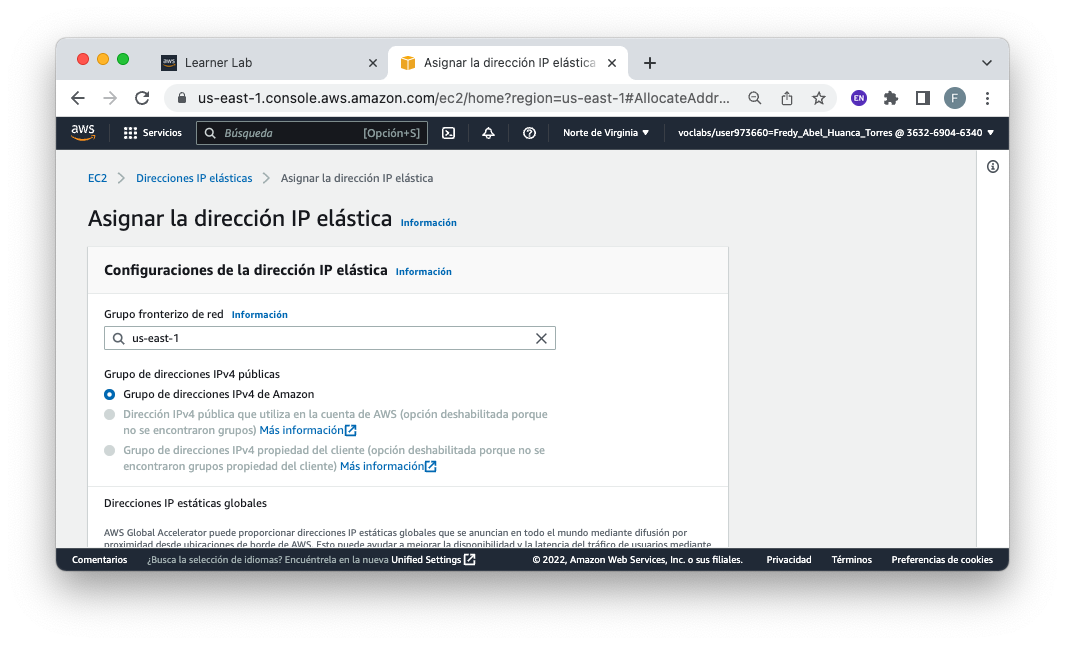
\includegraphics[scale=.35] {img/09-asignacionDeIpElastica}
	\caption{Instancia en ejecución}
	\label{fig:9}	
\end{figure} 

La siguiente figura muestra la asignación satisfactoria de un ip elástico asociado a la instancia ec2 que se muestra en la figura anterior.


\subsection{Asignación de IP elástica a la instancia}
\begin{figure}[h]
	\centering
	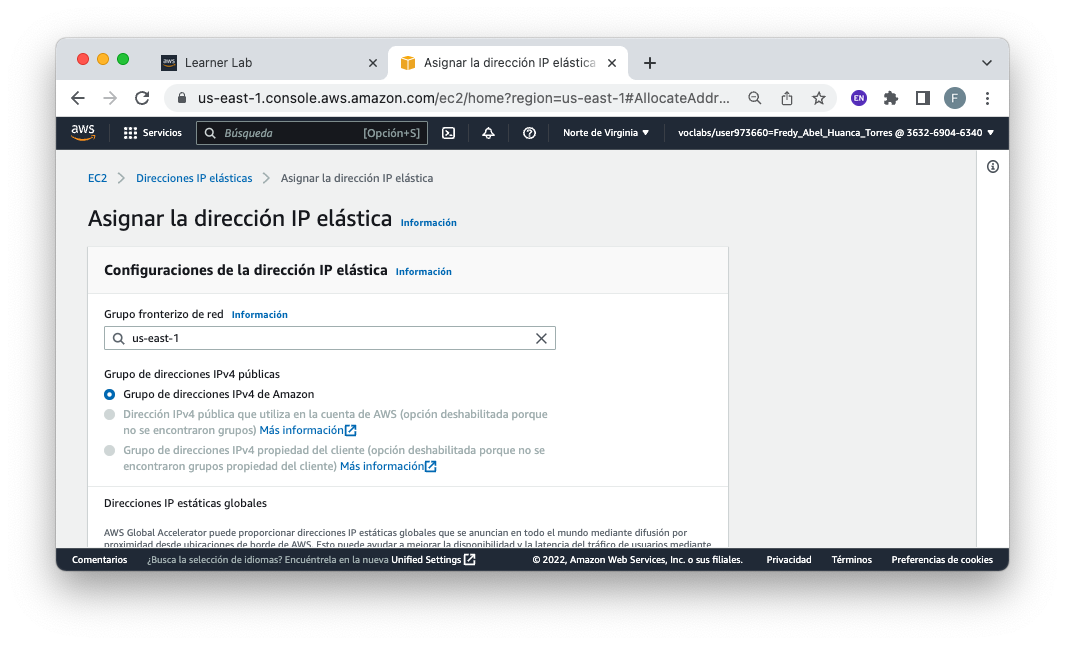
\includegraphics[scale=.35] {img/09-asignacionDeIpElastica}
	\caption{}
	\label{fig:9}	
\end{figure} 

\clearpage

\subsection{Asignación de IP elástica a la instancia}
\begin{figure}[h]
	\centering
	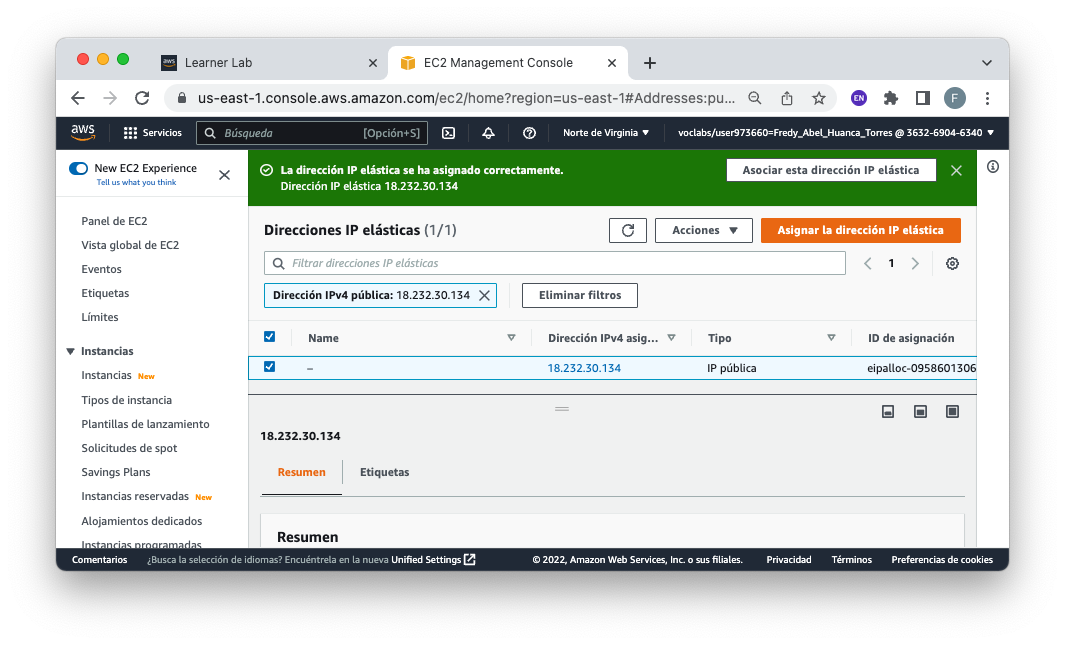
\includegraphics[scale=.35] {img/10-asigacionCorrectaIpElastica}
	\caption{}
	\label{fig:10}	
\end{figure} 

\subsection{Conexión segura por SSH}
Cambiando permisos de lectura y ejecución al archivo myKey.pem


\begin{figure}[h]
	\centering
	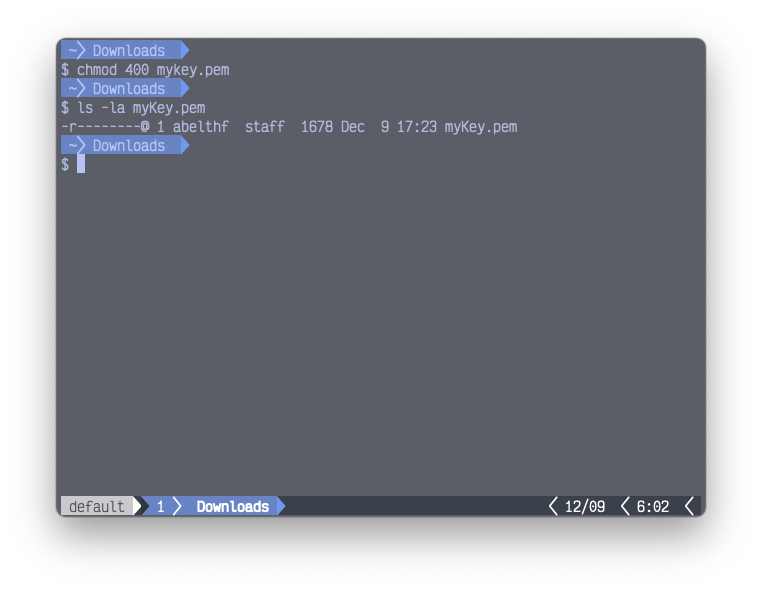
\includegraphics[scale=.35] {img/11-chmod400}
	\caption{Cambio de permisos}
	\label{fig:11}	
\end{figure} 

\begin{figure}[h]
	\centering
	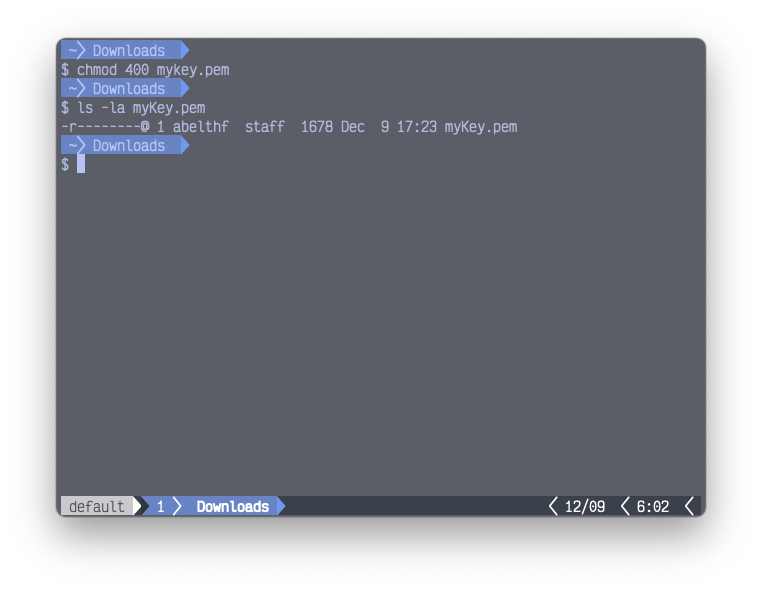
\includegraphics[scale=.35] {img/11-chmod400}
	\caption{Cambio de permisos}
	\label{fig:11}	
\end{figure} 

ssh -i mykey.pem ubuntu@44.192.119.93
 
fdsa
fdsa
fdas




Actualización de paquetes


Cambio de nombre al hostname

Instalación de OpenJDK


Descarga e instalación de Hadoop


Descompresión e instalación del instalador

cambiando y moviendo el paquete

Configuración del environment

Conexión segura por SSH

 

\subsection{Configuración de Hadoop}


-
-
-

\subsection{Inicio de Cluster de Hadoop}

-
-
-





\section{Ejemplo de Aplicación WordCount con Mapreduce}

\begin{sourcecode}[]{java}{WordCount en Java.}
import java.io.IOException;
import java.util.StringTokenizer;

import org.apache.hadoop.conf.Configuration;
import org.apache.hadoop.fs.Path;
import org.apache.hadoop.io.IntWritable;
import org.apache.hadoop.io.Text;
import org.apache.hadoop.mapreduce.Job;
import org.apache.hadoop.mapreduce.Mapper;
import org.apache.hadoop.mapreduce.Reducer;
import org.apache.hadoop.mapreduce.lib.input.FileInputFormat;
import org.apache.hadoop.mapreduce.lib.output.FileOutputFormat;

public class WordCount {

  public static class TokenizerMapper
       extends Mapper<Object, Text, Text, IntWritable>{

    private final static IntWritable one = new IntWritable(1);
    private Text word = new Text();

    public void map(Object key, Text value, Context context
                    ) throws IOException, InterruptedException {
      StringTokenizer itr = new StringTokenizer(value.toString());
      while (itr.hasMoreTokens()) {
        word.set(itr.nextToken());
        context.write(word, one);
      }
    }
  }

  public static class IntSumReducer
       extends Reducer<Text,IntWritable,Text,IntWritable> {
    private IntWritable result = new IntWritable();

    public void reduce(Text key, Iterable<IntWritable> values,
                       Context context
                       ) throws IOException, InterruptedException {
      int sum = 0;
      for (IntWritable val : values) {
        sum += val.get();
      }
      result.set(sum);
      context.write(key, result);
    }
  }

  public static void main(String[] args) throws Exception {
    Configuration conf = new Configuration();
    Job job = Job.getInstance(conf, "word count");
    job.setJarByClass(WordCount.class);
    job.setMapperClass(TokenizerMapper.class);
    job.setCombinerClass(IntSumReducer.class);
    job.setReducerClass(IntSumReducer.class);
    job.setOutputKeyClass(Text.class);
    job.setOutputValueClass(IntWritable.class);
    FileInputFormat.addInputPath(job, new Path(args[0]));
    FileOutputFormat.setOutputPath(job, new Path(args[1]));
    System.exit(job.waitForCompletion(true) ? 0 : 1);
  }
}
\end{sourcecode}


- Código Fuente

- Crear un archivo de entrada


- Crear un directorio en HDFS y copiar archivos de Local a HDFS


- Ejecución de MapReduce

- Salida



\section{Conclusiones}
% ------------------------------------------------------------------------------
% REFERENCIAS, revisar configuración \stylecitereferences
% ------------------------------------------------------------------------------
\clearpage
\bibliography{library} 